%% The following is a directive for TeXShop to indicate the main file
%%!TEX root = ../diss.tex

\chapter{Introduction}
\label{ch:introduction}

\begin{epigraph}
    \emph{
        What should I possibly have to tell you, oh venerable one? Perhaps that you're searching far too much? That in all that searching, you don't find the time for finding?
    } --- Siddhartha (1922), Hermann Hesse.
\end{epigraph}

\section{Activity Context}
\label{ch:introduction:sec:activitycontext}

In 1945 Vannevar Bush described the challenges to humans of
finding things in a codified system of records~\cite{bush1945we}:

\begin{quotation}
    \emph{Our ineptitude in getting at the record is largely
        caused by the artificiality of systems of indexing. When data of any
        sort are placed in storage, they are filed alphabetically or numerically, and
        information is found (when it is) by tracing it down from subclass to
        subclass. It can be in only one place, unless duplicates are used; one
        has to have rules as to which path will locate it, and the rules are
        cumbersome. Having found one item, moreover, one has to emerge from the
        system and re-enter on a new path.}

    \emph{
        The human mind does not work that way. It operates by association. With one
        item in its grasp, it snaps instantly to the next that is suggested by the
        association of thoughts, in accordance with some intricate web of trails
        carried by the cells of the brain. It has other characteristics, of course;
        trails that are not frequently followed are prone to fade, items are not
        fully permanent, memory is transitory. Yet the speed of action, the
        intricacy of trails, the detail of mental pictures, is awe-inspiring beyond
        all else in nature.}
\end{quotation}

This is as true in 2021 as it was in 1945.  Thus, the question that motivates my
research is: ``Can we build systems that get us closer to that ideal?''  My
argument that we can by capturing additional information that is not necessarily
useful to computers, but is useful to humans.

I call this additional captured information \emph{activity context}. While similar
to the ideas proposed in \emph{Burrito}~\cite{guo2012burrito}, I have broadened
that idea beyond just ``what a user is doing'' to incorporate information about
what the user is \emph{experiencing} that corresponds to more human-like context
information because it is useful for constructing \emph{association}.

Thus an ``activity context'' is an answer to the question:
\emph{what is going on in relation to the current event on a digital object?}
The job of the system becomes answering this question in a way that is useful.

More concretely, activity context is concerned with the environment in which a
given digital object is accessed.  Without restricting the abstract concept,
concrete examples of what I consider to be elements of an ``activity context''
might include:

\begin{itemize}
    \item Current weather.
    \item Notable news events.
    \item Focus website opened in a visible browser tab.
    \item User's mood.
    \item User's heart rate.
\end{itemize}

This is distinguished from \emph{what the digital object is}. While
understanding what something \emph{is} has merit, the context in which a digital
object is \emph{used} yields additional understanding about that digital object.

Further examples, in the form of ``use cases,'' can be found in
\autoref{ch:intro:sec:use-cases}.

\section{Thesis}
\label{ch:introduction:sec:thesis-statement}

\textbf{
    \input{thesis.tex}
}

\vspace{0.25cm}

``Intelligent use of files depends on having sufficient knowledge about them: their purposes, structures, and
contexts. Humans have traditionally made do by using their own methods for capturing and manipulating
such knowledge, but this is not available to programs, nor is it necessarily
convenient for humans~\cite{mogul1986representing}.''

Determining \emph{context} is a challenge with modern computer storage systems.
It is unrealistic to expect human users to provide that context.
Context is dynamic, imprecise, and not necessarily obvious, yet humans rely
upon context to create associations. By making environmental context information
available to programs, those same programs are able to present better options,
which \emph{is} convenient for humans.

%To improve the usefulness of naming systems within computer storage systems
%software must evolve to provide flexible, scalable, and multi-silo management
%of data object naming.


\section{Finding}
\label{ch:intro:sec:finding}

The volume of digital data is growing exponentially. Thus, it is not surprising
that solutions that worked when users were grappling with kilobytes (KB) or megabytes
(MB) of data do not work in the face of this growing deluge.

IBM's first magnetic disk drive could store up to 2.5
megabytes(MB)~\footnote{\url{https://www.7dayshop.com/blog/terabyte-evolution/}}
of digital data.  In 2020, we add 1.7MB of data \emph{per second per
    person}~\footnote{\url{https://techjury.net/blog/big-data-statistics/}}.  Today
we have become digital hoarders, collecting and keeping so much data that we often
cannot find specific objects when we need them.  How did we reach this point?

Early persistent storage systems used a simple flat directory structure
that gave a unique name to each object (``file'').  Such a simple structure was sufficient
to  name and identify distinct data objects (``files'').
\emph{Finding} the correct file was just a matter of scanning and picking from
the list.  This simple
structure did not scale well and was replaced by
a model based upon how paper documents were organized.
The hierarchical name
space~\cite{barnard1958,daley1965general,ritchie1973unix,Saltzer1978} is one in
which files (``digital objects'') are grouped into directories (sometimes called
folders).  Directories can also be grouped into other directories.  This model
mirrors how a filing cabinet works: multiple sheets of paper are gathered into a
folder, folders are organized into drawers, drawers into filing cabinets, filing
cabinets into rooms, etc. The directory and file metaphor was in use by
1958~\cite{barnard1958} and persists today as the common model despite the
volume of data being stored by a single computer storage device (``disk drive'') increasing by at least $10^6$~\footnote{Disk
    drives were measured in MB in 1965 and are measured in TB today.}.

In addition to the challenges of scaling, the file cabinet metaphor imposes
physical file limitations that are not valid for digital data.
Physical file cabinets do not allow a document to be in two folders at the same
time but there is no such restriction on electronic documents. The Multics
researchers addressed this by creating the \emph{link}, an idea that is
still used in many modern file systems~\cite{daley1965general}.

Computer networking enabled data sharing between users and computers but
complicated naming. Remote data access was typically represented to users either
as a hierarchical file system~\cite{nfs,howard1988scale} or an application program that programmatically
connected users to remote data~\cite{levin1979transport,10.1145/800216.806594,birrell1982grapevine}.

By 1990 the volume of data with which users interacted was so
large that researchers questioned the utility of the hierarchical name space~\cite{vicente1987assaying}.
The Semantic File System (SFS)~\cite{gifford1991semantic} suggested that
organization of digital objects be more fluid so that
users could group items together in ways that were semantically meaningful. The
meta-data generated from semantic information generated from file contents
permitted powerful query-based dynamic file organization.

While semantic file systems have not been widely adopted, the concept of
extracting semantic information from file content is present in modern file
indexing systems.  These indexing services employ ``transducers'' to extract
semantic information from files. Desktop search utilities (Windows
Search, Apple Spotlight, Station for Linux) rely upon indexing services to
provide their functionality.

\begin{figure}
    \centering
    \caption{First Wayback capture of google.com (google.stanford.edu) in 1998}
    \label{fig:google}
    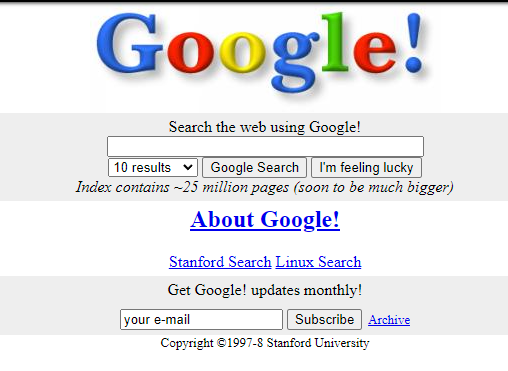
\includegraphics[width=0.95\textwidth]{figures/1998-11-11-Google-Screenshot-showing-early-index-size.png}
\end{figure}

There are parallels between the challenges of indexing files and the challenges
of indexing Internet web pages. Early search engines used a curation model in which
humans decided what websites were of interest based upon the information within
the web page itself --- similar to the way that semantic information was
extracted from files in the Semantic File
System~\footnote{\url{https://www.hpe.com/us/en/insights/articles/how-search-worked-before-google-1703.html}}.

Internet web page indexing changed profoundly when two Stanford graduate
students proposed a novel way to exploit the structure of Internet web pages to
extract \emph{usage} information from web pages that did not depend upon
semantic content~\cite{page1999pagerank}.

Google's website used to state the number of pages that they indexed.  In 1998
the first capture of Google's website by archive.org shows they claimed to index
more than 25 million pages (\autoref{fig:google}). Google no longer publishes
that number but industry estimates indicate the number is at least $10^3$ more
now than it was then, and this only covers a few percent of the entire content
stored on the
Internet~\cite{bosch2016estimating}~\footnote{\url{https://www.worldwidewebsize.com/}}.

Could we utilize a similar technique for finding information within our own
trove of files? While there are similarities between the Internet and our file
collections, there are also significant differences. Files lack the level of common
structure present in web pages, preventing simple extraction of references
between files. Files (or digital objects) are stored in myriad
locations with different access mechanisms: local storage, cloud storage,
database, collaboration applications, e-mail programs, etc.  Sometimes these
overlap: your e-mail program stores some or all of your data on your local
computer, within your local storage. However, you do not expect to use the tools
for searching your local storage to find things within your e-mail software.
Thus, we should consider them to be distinct storage locations. I refer to these
distinct storage locations as \emph{storage silos} (or just \emph{silos}) to
emphasize their inherently separated nature.

Network storage is presented in many different formats: an inexpensive disk
drive attached to the local network represents ``Network Attached Storage''
(NAS) or a specialized parallel data cluster such as HDFS~\footnote{\url{https://hadoop.apache.org/docs/r1.2.1/hdfs_design.html}},
DAOS~\footnote{\url{https://www.intel.ca/content/www/ca/en/high-performance-computing/daos-high-performance-storage-brief.html}},
Lustre~\footnote{\url{https://www.lustre.org/}}, or
Ceph~\footnote{\url{https://docs.ceph.com/en/pacific/cephfs/index.html}}.
They typically support one or
more common data sharing protocols, such as NFS~\cite{sandberg1986sun} or
CIFS~\footnote{\url{https://docs.microsoft.com/en-us/openspecs/windows_protocols/ms-cifs/d416ff7c-c536-406e-a951-4f04b2fd1d2b}}.
They vary dramatically in how they are managed, accessed, and searched.  In most
cases there is no common interface --- each represents a unique ``storage
silo.''

Cloud storage is one specific type of network storage that is popular because it
allows you to access your data from any of your devices, provides a reliable
backup mechanism, and permits selective download to any given device. However,
these benefits are paired with challenges when it comes to finding specific
digital objects.  If files are not present on your local device, the indexing
services on those devices cannot assist you.  You could download all of the
content from the cloud storage providers to enable indexing, but that consumes
considerably more bandwidth and storage and is impractical for devices that have
resource constraints.  While we can use the cloud providers' search services, that
requires iteration over each of those services, using different interfaces with
variable results.

Our files come from multiple sources including websites, e-mails, databases,
and collaboration tools.  Those documents are stored both locally and remotely.
We create, access, and modify documents and then send them onwards using any of
the variety of silos and collaboration tools at our disposal.  Just a few days
after we last accessed them we struggle to find those
documents.

Given the diffusion of files across storage silos that occurs because of our
sharing and use, we often find versions and related files scattered across
multiple silos. We struggle to find these versions and determine when we have
found the ``right'' one.

Returning to the question of using contextual information for improving
\emph{finding}, the research community has observed that adding
contextual information, such as the current weather, to existing file
collections materially improves human ability to find the relevant digital
object~\cite{vianna2019thesis,10.1145/1559845.1559992,dumais2016stuff}. Thus, it
seems the answer is ``Yes, using contextual information improves
\emph{finding}.''

Google solves a simpler problem: an Internet web search need merely find
\emph{an} answer to the search query.  A personal file search needs provide
\emph{the} answer. Thus, it may not be possible to provide a definitive answer,
but narrowing the potential list of plausible answers leads users to the
relevant file, which is the goal of \emph{finding}.

The data that we need for creating activity context is already being collected
by our computers. Modern computers collect vast amounts of information about us:
what we do, where we are, with whom we communicate, the applications we use, the
files we access, the music we play, the web pages we visit, even how we
feel~\cite{chakriswaran2019emotion,8933554}.  We \emph{know} this
data exists because our own devices provide this information to third parties.
Given this data is already being collected, we know the additional cost will be
to store and make it accessible to applications.

\emph{Finding as a Service} (FaaS) will use this existing information to solve our data
finding problem. FaaS decouples \emph{finding} objects from \emph{storing}
objects.  FaaS facilitates \emph{finding} by exploiting contextual information
beyond the basic object characteristics widely available for searching today:
names, types, and dates. By relating information we already have with how our
digital objects are used, we provide the \emph{activity context} to enable
\emph{Finding as a Service} (FaaS).

\emph{Activity context} is important because it captures useful
information about the environment in which files are created,
consumed, and updated.  \emph{Activity context} need not be something the system
ordinarily relates to the digital object.  \emph{Activity context} captures key
information about the the user's wholistic environment.

\section{Use Cases}
\label{ch:intro:sec:use-cases}

The following use cases provide specific scenarios that cannot be
achieved using current systems.  I maintain that \emph{Finding as a Service}
addresses these use cases, which supports my thesis.

\begin{itemize}
    \item \label{use-case:e-mail}\textbf{The lost original.} Imagine that you received a spreadsheet
          from someone.  You begin to edit it, add information, sift through it.  At
          some point you realize that you sorted a subset of the columns, hopelessly
          scrambling the original information and your edits. You try to find the
          original source of the spreadsheet, only to realize that you cannot do so,
          even when you search in your e-mail program using the \emph{name} of the
          file that was saved on your local drive as part of your editing process. The
          system should permit you to find the original source of the information,
          even though the related digital objects are in different \emph{silos}.

    \item \label{use-case:misplaced-presentation}\textbf{The misplaced presentation.} You arrive at a meeting with your
          client after a long trip, only to realize the laptop computer you were
          using will not boot.  You have your smart phone and you \emph{think}
          you saved it to a cloud service.  How do you find it so you can share
          it with a colleague at the meeting? The system should permit you to
          find your own digital data in your cloud storage regardless of which
          device you used to create it.

    \item \label{use-case:multi-silo-problem}\textbf{The multi-silo relationship problem.} A colleague shares their
          experimental data with you, which was stored in NREL's
          High-Performance Computing Data
          Center~\footnote{\url{https://www.nrel.gov/computational-science/hpc-data-center.html}}.
          You then use that data as part of your own work, which you wish to
          share with a broader audience using Compute
          Canada~\footnote{\url{https://www.computecanada.ca/techrenewal/rdm/}}.
          You also shared your computational notebooks using your organization's
          account with Microsoft~\footnote{\url{https://visualstudio.microsoft.com/vs/features/notebooks-at-microsoft/}}.
          You created your slides in
          Prezi~\footnote{prezi.com} and presented them to a different research
          group on their Discord server~\footnote{\url{discord.com}}. One of the
          people that attended downloaded two of your notebooks and created a
          new notebook from them.  They then shared that notebook publicly via
          Google Colab~\footnote{\url{https://colab.research.google.com/}}.
          Your colleague knows that she shared her data with you and wants to be
          able to quickly find the documents that you and others have shared
          based upon that original data. Collaborative work like this is a
          modern reality and it is unlikely that all work product will be co-located.
          The system should permit your colleagues to find the work you and
          others have shared with her \emph{without} your intervention.

    \item \label{use-case:multi-silo-finding}\textbf{Multi-silo finding.} \persd is a visiting student from the
          country of Lemuria doing an internship with you in Camelot.  While arranging
          for this internship, \persd required \emph{numerous} different data objects:
          email messages with the host, offer letters, academic forms, a visa,
          boarding passes, project proposals, and more. The system should be able to
          provide you with a set of related files, regardless of their storage
          silo.

    \item \label{use-case:info-source}\textbf{The where did I get this information conundrum.}  In our modern
          world we often have one (or more) web pages open when we are authoring one
          (or more) documents.  A reasonable question to ask would then be ``what web
          pages did I look at while writing this document?'' Often it is not just that
          you looked at a given web page, but also if it was the last web page you
          looked at and how long you looked at it.  The system should be able to
          provide you with a list of that web activity.

    \item \label{use-case:privacy}\textbf{How do I share information while
              preserving privacy?} \persg, an investigative journalist who routinely receives
          sensitive information
          from third parties, is investigating the company from the prior use cases.
          \persg needs to be able store and access sensitive information, including
          information about the activity context of various e-mails, documents, pictures,
          and audio and video files. While \persg ensures that these data are
          encrypted, they need to also ensure
          that they can both find information and ensure that meta-data associated with
          those files is both usable and properly protected across silos.
          While \persg must protect their sources, they must also be able to associate
          evidence with those sources to make judgement calls about their validity.
          The system should support security and privacy policies for attributes that
          accomplish both.
\end{itemize}

This list of use cases is not exhaustive and is intended to provide cases that
resonate with readers.  They are use cases that are not addressed by existing
systems.  I review these existing systems and how they fail to address these use
cases in \autoref{ch:intro:sec:existing-solutions}.

\section{Existing Solutions Fall Short}
\label{ch:intro:sec:existing-solutions}

Prior work has addressed some of the challenges that I identified in the use
cases (\autoref{ch:intro:sec:use-cases}).  I briefly introduce key
aspects of how they fall short here and provide greater detail in
\autoref{ch:background}.

A simple solution to the multi-silo namespace challenge is to graft those
namespaces together. UNIX mount points~\cite{unix} are perhaps the first
instance of such federating namespaces. Distributed federation, as provided by
distributed file systems such as NFS~\cite{nfs} and AFS~\cite{howard1988scale}
emerged in the 1980s soon after adoption of high speed networks such as
Ethernet~\cite{digital1980ethernet}.

There is some work in cloud storage federated
namespaces~\cite{scfs,federatedMetaData}.
Nextcloud~\footnote{\url{https://nextcloud.com}} allows users to connect
multiple Nextcloud instances and integrate with FTP, CIFS, NFS and object
stores. This yields a classic hierarchical namespace structure with its known
limitations~\cite{vicente1987assaying,vicente1988accommodating}. It does nothing
to facilitate \emph{finding}. Peer-to-peer sharing networks (e.g., IPFS \cite{benet2014ipfs}) implement a
distributed file system where nodes advertise their files to users.
MetaStorage~\cite{metastorage} implements a highly available, distributed hash
table, similar to Amazon's DynamoDB~\cite{10.1145/2213836.2213945},
but with its data replicated and distributed across different cloud providers.
MetaStore offers a key-value store interface~\footnote{\url{https://cwiki.apache.org/confluence/display/hive/design}}.
Farsite~\cite{Adya:2003:Farsite} organizes multiple machines into virtual file
servers, each of which acts as the root of a distributed file system. Comet
describes a cloud oriented federated metadata service~\cite{federatedMetaData}.

None of these address the scaling problem that arises when data is analyzed and indexed
away from where it is stored.  Similarly, none of these address the integration
of sensitive locally stored information about personal usage of these objects.
Thus, one key benefit of better \emph{finding} is that
it should improve the efficiency of retrieving data stored across non-local
storage silos.

Some prior work explored using extrinsic usage information for \emph{finding}.
Placeless~\cite{placeless-tois} focused on using process level information extracted from their document processing
system to associate files together. Similarly,
Burrito~\cite{guo2012burrito} proposed \emph{activity context}, which they define as ``the
user's actions at a particular time.'' Both look at narrow instances of the
larger \emph{finding} problem.

Provenance uses observable information about construction of a file to augment file
search, which in turn improves findability~\cite{provsearch}. Provenance search
takes a narrow view of the activities of interest and are all largely
\emph{causality} focused.  However, humans tend to think
associatively~\cite{10.1145/1559845.1559992}, focusing on what else was
happening --- the cleaning crew came by their desk while they were writing that
document, the discussion at a meeting with others, their location when they
wrote a given document, or some other event that was happening around the time
they interacted with a given document.

While environmental information is not as obviously related as causal
relationships, prior work related to using statistical inference to establish
relationships within the storage domain has demonstrated such mechanisms can be
more efficient at identifying patterns that lead to higher
efficiency~\cite{10.1145/3035918.3064029}.

\section{Contributions}
\label{ch:intro:sec:contributions}

The research to support my thesis will contribute the following:

\begin{enumerate}
    \item Production of the \emph{Finding as a Service} (FaaS) dataset, a
          collection of meta-data and activity context from a local system, that
          will enable me to explore potentially useful information for informing
          activity context data collection. In addition, I will publicly
          share this data set to enable other researchers to develop new
          techniques for users to find digital items.

    \item \system~\footnote{\system is Xhosa for pragmatics.  In Linguistics,
              pragmatics is the study of meaning within a given context}, my
          architecture for a system that captures, stores, and
          disseminates \emph{activity context} without imposing excessive resource
          demand.

    \item \systemone~\footnote{\systemone is the Uzbek word for finding; the most
              recent graduate student from our research group is from Uzbekistan and
              has always been supportive of my research}, a single node
          implementation consistent with \system that provides
          \emph{FaaS} across multiple storage silos on a single
          system.

    \item \systemtwo~\footnote{\systemtwo is the Russian word for finding in
              recognition of the support for my research that I have received from both Ada Gavrilovska and
              Alexandra Fedorova.}, a distributed implementation of \system that provides
          \emph{Finding as a Service} (FaaS) across multiple systems using a
          combination of device private and cross-device shared storage
          silos.

    \item An evaluation demonstrating that it is possible to capture activity
          context without imposing excessive overhead, in either space or time.

\end{enumerate}

These projects focus on improving \emph{finding}.

The remainder of this document provides more specific insight into these
contributions and how I propose creating and disseminating them.
In \autoref{ch:background} I review the prior work that
underlies my thesis: what types of storage silos exist, what information we
already have available and why these are not sufficient to meet these use cases.
In \autoref{ch:research-questions} I set out the research questions that I
seek to answer to fully explore my thesis.
In  \autoref{ch:architecture} I describe the structure of the system I
propose building in order to support my thesis and how it addresses these use
cases.  In \autoref{ch:evaluation} I discuss how I propose evaluating
my system.  Specifically I attempt to address key questions, such as: ``how well does it address these use cases?'', ``what are the performance
and resource implications of using my system?'', and ``how well does it enable other
communities to construct more effective finding tools?''

\endinput

\section{Meeting Notes}
\tm{This section is to be removed.  It is my recording of notes from the meeting of October 19, 2021 with Margo and Sasha.}

The vast majority of prior work has focused on using properties that are
intrinsic to the file to facilitate search and naming and in large part this
project is about looking outside the file and including environmental
information which we call ``activity context.''

That leads to the story line that says if we look at how we have both

Differentiate \emph{naming} from \emph{finding}. We've always been talking about
this as \emph{naming} and I'm no longer convinced that we are solving a naming
problem, I feel that we are solving a \emph{finding} problem.

There's this nice linear history.  We start with the hierarchical name space.
It was a way to organize digital information in a manner that reflected physical
data organization.  Gifford points out that the digital world offers us a richer
space and therefore when we consider these intrinsic attributes we can
facilitate even better finding.  There have been \emph{hints} that expanding to
looking at factors outside the file might provide an improved experience.  That
is Guo [Burrito] and Soules [Provenance Search].  We are taking that hint of an
observation and broadening it into something we all ``activity context'' which
is about the environment in which an object exists and here are examples of the
kinds of queries that we want such a system to be able to satisfy.

\item The prior work suggests context helps (cite Soules).  We want to
enable HCI researchers to ask the broader question of whether broadening the
definition of environment [activity context] also helps.  We do not want to
\emph{answer} that question --- we want to enable a system that permits the
HCI research community to explore it.  To do that, we need to identify how
you get this information.

That then begs several research questions:

\begin{itemize}

    \item What events are useful in establishing relationships between objects?
          I might suggest the question you want to ask is ``What is the universe of
          relationships that I can extract and how can I do that?''  Then we can ask
          to the HCI researchers to ask them which would be of interest to them.
          ``What is the universe of relationships that we could extract?'' and ``what
          are the techniques that we need to develop to extract them.''  At some point
          we have to introduce this multi-silo world, but let's hold off.

    \item We would like to build an extensible framework that allows you to add
          all these things.  What we have discussed in the past is another mode for
          getting this internal information, which is ``I pipe it through the ML
          service, which indicates if there is a cat in it, or not.'' [Note that in
          the extrinsic view, this isn't interesting because the ML classifier is just
          another form of transducer].

          Your description of what one needs to do is largely spot on (from the
          spreadsheet).  I would hesitate to call this ``the thesis question''; as a
          systems researcher identify all the things that I can collect already and
          then develop a framework that makes it easy to add other things and then
          another piece where we bring them together in the multiple silo thing.

          Notice you can in fact do a bunch of this in a single silo; you can do this
          for a single system by broadening Guo and Soules work and saying ``ok we
          really want to capture''.  I'd go back and look at Guo carefully that even
          in the single systems world I think his work captures all the things we're
          talking about but it is worth going over it carefully and making sure of
          that.

              [Sasha typed] ``The current silos are conventional ones can we think about
          something that one might not think of as a silo?''  Discord, slack, e-mail
          are all silos.  \emph{Those are frustrating silos}. ``What I was browsing at
          a particular time.''  Two different dimensions here: the different kinds of
          silos and

          In the background chapter it is worth enumerating all these different silos
          (the ones we can think of) and going from obvious to crazy.

          The other dimension, the kinds of environmental factors we might want to
          think about.  What was I browsing, what was I listening to, what other
          documents were open, did I move the browser tab to a different window [how
                  long did I spend looking at the given tab - e.g., ``how long did this tab
                  have focus'' for example].

          Do we try to capture everything?  Winnowing process.

          Sasha: I have a thought on how this could easily turn into a systems
          problem.  We could try to categorize alll kinds of crazy silos,
          applications, activity contexts with respect to how we can collect their
          information.  For example, conventional things like chat and discord we just
          go into their meta-data.  Things like file systems we go into their files
          and file names.  More crazy things like ``what I was browsing'' we might
          need to capture screen or capture charactters.  Have a categorization of
          techniques for collecting activity context such as browser search and meta
          data versus capturing the screen versus something else. The categorization
          of silos and see how they match.  Which silos work with which methods.
          Where do we need to invent new methods.  This then leads to the question
          like the amount of data and parsing it and storing it and that quickly turns
          into a systems problem.

          ``What is the information?''
          ``How can we capture it?''
          ``What is the service that unifies this information and makes it
          available/usable?''



\end{itemize}

This is the diagram from the white board:

\begin{itemize}
\item Introduction
\begin{itemize}
    \item Linear history
          \begin{itemize}
              \item HNS
              \item SFS
              \item TFS [Tony FS].
          \end{itemize}

    \item Background
          \begin{itemize}
              \item Silos (Taxonomy).  Classification of silos that let you collect data.
                    \begin{itemize}
                        \item What can you collect?
                        \item How can you collect?
                    \end{itemize}

                    We need HCI feedback on this information.  Helps us focus our initial
                    data collection effort to focus on selecting data that is useful to
                    them.

                        [Margo] Asking them what they want means we are limited to the things
                    they can imagine.  Thus, we need to have a universe of things that we
                    can offer them. [TM: there are integration components already for quite
                            a range of applications. E.g., discord integrates with games, music
                            players integrate with other stuff as well]
          \end{itemize}

    \item Architecture

          How do you integrate info into a service?  ``Context as a Service'' (CaaS).
          This is Kwishut so start by lifting that work.

    \item Privacy/Security

          We agreed that \emph{security} is not really the core issue for this system:
          we aren't subverting the existing system, we aren't proposing some bypass
          for the existing system.  Thus, the security consideration is largely about
          protecting our own meta-data.  There are standard techniques for doing
          authentication that can be used for connecting from a client to a trusted
          server, there is no need for us to re-invent the wheel.  By deliberately
          designing the system so that activity context information is maintained on a
          trusted machine, whether local or remote, we can assert that it is \emph{by
              design} secure.  Similarly, by restricting access to only a trusted machine
          the system ensures privacy as well since only authorized agents can access
          the activity context.  This does not exclude the possibility of having
          different architectures for data sharing.

          Worrying about securing the system at this point is premature: a generalized
          multi-tenant activity context system could be useful for correlating
          activities across users and systems, but is premature until we have
          established that activity context is itself useful.

              [Shasha] I wonder if we are inventing a new type of privacy paradigm on a
          local device.  What we have right now is when I'm setting up my new
          device each app asks me what is allowed or not allowed.  Here, I want
          something else: I want to allow it as long as the information stays on
          the device and is for my personal use, or allowed by certain
          applications, but I don't allow it to leave the device, or to allow it
          to be exfiltrated but only if it is encrypted.

          Kosta in ECE usable privacy/security.  He will probably be able to
          point to related work and decide what to do with it.  Use it to
          prepare for responding to the issue.

              [Margo] extract from the draft, get it to him before the presentation
          could have more information to share at the presentation.

    \item Evaluation

          We show this data is useful because the HCI researchers have confirmed it is
          useful.  Now the evaluation will fall out: lots of data, difficult to gather
          it, how you store it, model it, query it.  How to build this thing and make
          it useful.  Each one of these items will have an evaluation piece.

          How do I enable query?  Here's the interface I'm going to do and here
          is how that addresses these N use cases that we presented that you
          can't do in other systems.  These are use cases that we hypothesize
          are useful and you can't do them today and here's how you do them with
          this proposed system.  The overhead: massive amounts of data, how do
          we manage it.  What is the size, what is the performance impact.  How
          easy is it to add another silo?  These metrics can be used to evaluate
          the system we're proposing to build.

          The efficacy comes down to ``assuming that we have got some HCI
          researchers off looking at the data we collected initially, by the
          time we have built a system we ought to be able to just re-run that
          evaluation across multiple silos with this distributed data.''

          The storyline for the thesis has to be this is about building a system
          to facilitate this other world.  We are hoping that we will have
          collaborators to do that and are actively pursuing them.  My question
          is ``assuming it is useful, can we even build such a system that will
          enable that?''

\end{itemize}

[Sasha]  Write the intro and background from scratch, watch the recording,
transcribe what you said and you'll have most of the background.

